\documentclass{article}
\usepackage{amsmath,amsfonts,amsthm,amssymb,chemformula,fullpage,graphicx,multicol,multirow,parskip,setspace}
\usepackage[backend=biber,sorting=none,style=numeric-comp,giveninits]{biblatex}
\usepackage[colorlinks=true,citecolor=blue,linkcolor=black,urlcolor=blue]{hyperref}

\DeclareNameAlias{default}{family-given}
\renewbibmacro{in:}{}
\addbibresource{references.bib}

\onehalfspacing

\title{MAT 541 001 Modern Algebra\\Molecular Symmetry and Group Theory}
\author{Maggie Barker}
\date{December 1, 2025 (second draft)}

\begin{document}
    \maketitle

    \tableofcontents

    \section{Introduction}

    Symmetry is a bridge that connects the world that we can see with the quantum mechanical realm that governs the laws of chemistry. The language that describes symmetry is that of mathematics, in particular group theory, representation theory, and character theory. Countless chemical processes are connected to the symmetry of molecules, and a deep understanding of these concepts is rooted in algebra. In this paper, we will take a interdisciplinary tour of this interface between chemistry and mathematics. First, we will introduce some basic chemistry principles that will aid in understanding. We will look at the symmetry that molecules possess and how to categorize it in a systematic fashion via point groups. Then we will switch to a mathematical discussion of groups, matrices, and characters, and learn how to build character tables for point groups from scratch. Then we will switch back to chemistry and discuss the interplay of symmetry and molecular vibrations. Finally, we will look at a few applications of character theory in chemistry. Much of the presentation of point groups and character theory follows the treatments in \cite{miessler2014,mcgrady2024,vallance,young}.


    \section{Brief review of chemical structures}

    At the submicroscopic level, all matter is composed of atoms, which are further broken into protons, neutrons, and electrons. Protons have positive charge, neutrons have no charge, and electrons have negative charge. Protons and neutrons are clustered together in the nucleus, a dense ball in the center of the atom. Electrons surround the nucleus in orbitals, which can be thought of as probabilistic ``clouds'' where the electrons are most likely to be at any given time. The identity of a particular atom (e.g., carbon, oxygen, etc.) is fully determined by the number of protons in its nucleus. Atoms can exist independently, but most of the matter we encounter on a daily basis is not made of individual atoms, but rather clusters of atoms in the form of molecules or ionic compounds.

    Atoms \emph{bond} together through interactions of their electrons. The driving force of the bonding process is stability; atoms are in their most stable state when their outermost orbital is completely filled with electrons. Atoms can either gain or lose electrons in order to achieve this stable state. When two atoms share electrons more or less equally with one another, we have a covalent bond. When one atom takes the electrons entirely from another atom, we have an ionic bond. Ionic bonds occur in table salt (\ch{NaCl}), for example. We will be focusing instead on \emph{molecules}, which are clusters of atoms that are covalently bonded with one another. Molecules exist in myriad fascinating ways, from simple molecules like \ch{H2O} to incredibly complicated molecules like DNA. Our main focus will be on characterizing the symmetry of simple molecules, although the process involved can be extended to more complicated cases.

    When two electrons are shared between two atoms, we have a single bond, denoted as \ch{C-C}, for example. When four electrons are shared, we have a double bond, denoted \ch{C=C}. When six electrons are shared, we have a triple bond, denoted \ch{C+C}. Components of molecules can freely rotate along the axis of a single bond, but double and triple bonds are locked and cannot rotate.

    To understand the shapes of molecules, it is essential to learn a little bit of VSEPR theory. VSEPR (``VES-per'') stands for Valence Shell Electron Pair Repulsion. For this purpose, we will choose one atom in a molecule to be the central atom. (For the simple molecules we deal with, the central atom will be apparent visually.) The name of VSEPR itself explains a lot of the theory. The valence shell is the outermost orbital of electrons, where bonding takes place; electrons tend to occur in pairs; like charges repel, so electron pairs tend to position themselves to be as far away from other electron pairs as possible. Now, some of the electron pairs on the central atom will be bonding (shared with other atoms), and some will be nonbonding (not shared). A pair of nonbonding electrons is called a \emph{lone pair}.
    
    \begin{figure}[htbp]
        \centering
        \includegraphics[width=5in]{vsepr.jpg}
        \caption{The most common molecular geometries based on VSEPR theory. \cite{chemlearner}}
        \label{fig:vsepr}
    \end{figure}

    The number of electron groups is the sum of the number of bonds and the number of lone pairs on the central atom. (For this purpose, single, double, and triple bonds are treated equally.) The number of electron groups and the number of lone pairs is all that is needed to determine the \emph{molecular geometry}, as shown in Figure \ref{fig:vsepr}. In water (\ch{H2O}), the oxygen atom is bonded to two hydrogen atoms and has two lone pairs. Hence, water is a bent molecule. In ammonia (\ch{NH3}), the nitrogen atom is bonded to three hydrogen atoms and has one lone pair. Therefore, ammonia is a trigonal pyramidal molecule. In methane (\ch{CH4}), the carbon atom is bonded to four hydrogen atoms and has no lone pairs. Thus, methane is a tetrahedral molecule.

    As mentioned above, the sharing of electrons between atoms in a covalent bond can be more or less equal. If the atoms are of similar ``strength'' (similar electronegativity), the electrons will be shared equally, forming a nonpolar bond. If one atom is ``stronger'' than another (higher electronegativity), it will attract electrons to it, causing the sharing to be unequal. This results in a polar bond. If the polar bonds are equal and in opposite directions, they cancel by \emph{symmetry}, and the molecule will be \emph{nonpolar}. This occurs in carbon dioxide (\ch{CO2}), which is a linear molecule (C has two double bonds, no lone pairs). By contrast, if the polar bonds do not cancel by symmetry, the molecule will be \emph{polar}. This occurs in water. Many of the interesting characteristics of water (high boiling point, high surface tension, ice having a lower density that liquid water, etc.) are a direct consequence of the strong hydrogen bonds formed between different water molecules, and this is due to the polarity of the water molecule. If water were nonpolar, it would most likely be a gas at room temperature and behave more like carbon dioxide or methane. Life as we know it would be impossible if water was not a bent polar molecule!

    \subsection{Notes about notation}

    For the sake of representing three dimensional molecules on two dimensional paper, some bonds will be drawn as wedges and dashes. For example, consider the following molecule:
    
    \begin{center}\includegraphics[width=1in]{c1example.jpg}\end{center}

    Here, the wedge bond implies that the chlorine (Cl) atom is facing towards the reader, while the dashed bond implies that the bromine (Br) atom is facing away from the reader. The normal (skinny) bonds should be interpreted as being in the plane of the paper.

    One other convention that needs to be noted is the way benzene rings will be shown. Benzene is a ring of six carbons with alternating (conjugated) double and single bonds, with each carbon bound to a hydrogen, as follows:

    \begin{center}\includegraphics[width=1in]{benzene.jpg}\end{center}

    Due to the tedious nature of drawing this molecule and its frequency of occurrence, it will be shown in the following standard shorthand way:
    
    \begin{center}\includegraphics[width=0.5in]{d6hexample.jpg}\end{center}

    \section{Symmetry elements and operations}

    Many molecules contain \emph{symmetry elements}, such as rotational axes, mirror planes, and inversion centers, upon which \emph{symmetry operations} can be performed, such as rotation, reflection, or inversion. The molecule will be indistinguishable before and after the symmetry operation.

    The most basic symmetry operation is $E$, the identity operation. This is the act of doing nothing, and is required in order to express a collection of symmetries as a group.

    A proper rotation, $C_n$, is a rotation that can actually be achieved in three-dimensional space. It is a rotation through $360^\circ/n$ counterclockwise with respect to some axis. We have that $C_n^n\equiv E$, so that the order of the rotation $C_n$ is $n$. If a molecule has more than one rotational axis, the one of highest order is called the \emph{principal axis}. By convention, a $C_2$ axis will be denoted $C_2'$ if it passes \emph{through} outer atoms, and $C_2''$ if it passes \emph{between} outer atoms.

    A reflection over a mirror plane is denoted $\sigma$. In particular, a reflection plane that is perpendicular to the principal axis is called horizontal and denoted $\sigma_h$. A reflection plane that includes the principal axis is called vertical and denoted $\sigma_v$. A vertical reflection plane that bisects the angle between two $C_2$ axes is called dihedral and denoted $\sigma_d$.

    The inversion operation, $i$, is where every point of the molecule is moved through the inversion center (the center of the molecule) to its opposite position the same distance from the center.

    An improper rotation, $S_n$, also called a rotation-reflection, is a $C_n$ rotation followed by a $\sigma_h$ reflection through a plane perpendicular to the rotation axis. Two $S_n$ operations together form a $C_{n/2}$ operation. An $S_2$ operation is equivalent to $i$. In some molecules, $S_j$ axes are coincident with $C_k$ axes.

    \section{Point groups}

    The collection of symmetry operations that a molecule possesses determines its \emph{point group}. It is named such since every symmetry element shares a single point. \cite{johnston2014} Determining the point group of a molecule can be rather complicated, but there is a sequence of steps that can be followed to determine a point group without much trouble. To get started, we can classify molecules as being of \emph{low symmetry}, \emph{high symmetry}, or neither. We will list the point groups of the three categories and show example molecules that exhibit each group. To assist in determining the point groups for molecules of neither low nor high symmetry, we will use a flowchart.

    \subsection{Point groups of low symmetry}

    Molecules in the $C_1$ group have no symmetry besides the identity operation $E$. (Indeed, every point group contains $E$, but it will not be mentioned in the following groups.)

    \begin{center}\includegraphics[width=1in]{c1example.jpg}\end{center}
    \pagebreak

    Molecules in the $C_s$ group have only one mirror plane (in the following example, the mirror plane is the plane of the molecule).

    \begin{center}\includegraphics[width=1in]{csexample.jpg}\end{center}

    Molecules in the $C_i$ group have only an inversion center.

    \begin{center}\includegraphics[width=1in]{ciexample.jpg}\end{center}

    \subsection{Point groups of high symmetry}

    Molecules in the $C_{\infty v}$ group are linear, with infinite rotation order and an infinite number of reflection planes containing the rotation axis. They contain no inversion center. An example is hydrogen chloride.

    \begin{center}\includegraphics[width=1in]{cinfvexample.jpg}\end{center}

    Molecules in the $D_{\infty h}$ group are like $C_{\infty v}$, but with perpendicular $C_2$ axes, a perpendicular mirror plane, and an inversion center. An example is carbon dioxide.

    \begin{center}\includegraphics[width=1in]{dinfhexample.jpg}\end{center}

    Molecules in the $T_d$ group are tetrahedral, with four $C_3$ axes, three $C_2$ axes, three $S_4$ axes, and six $\sigma_d$ mirror planes. An example is methane.

    \begin{center}\includegraphics[width=1in]{tdexample.jpg}\end{center}

    Molecules in the $O_h$ group are octahedral, with 48 symmetry operations in all. An example is sulfur hexafluoride.

    \begin{center}\includegraphics[width=1in]{ohexample.jpg}\end{center}
    \pagebreak

    Molecules in the $I_h$ group are icosahedral, with 120 symmetry operations in all. A fascinating example is buckminsterfullerene, a molecule with sixty carbon atoms in a soccer ball shape.
    
    \begin{center}\includegraphics[width=1in]{bucky.png}\end{center}

    \subsection{Other point groups}

    To help distinguish which molecules are in each of the remaining point groups, we can refer to the flowchart in Figure \ref{fig:flowchart}.

    \begin{figure}[htb]
        \centering
        \includegraphics[width=6.5in]{flowchart.png}
        \caption{Flowchart to help determine point groups of molecules.}
        \label{fig:flowchart}
    \end{figure}
    \pagebreak

    Molecules in the $C_{nh}$ group contain a $C_n$ rotation axis, a horizontal mirror plane $\sigma_h$, and an inversion center. The following examples are $C_{2h}$, $C_{2h}$, and $C_{3h}$, respectively:

    \begin{center}\includegraphics[width=1in]{c2hexample1.jpg}\includegraphics[width=1in]{c2hexample2.jpg}\includegraphics[width=1in]{c3hexample.jpg}\end{center}

    Molecules in the $C_{nv}$ group contain a $C_n$ rotation axis and $n$ vertical mirror planes $\sigma_v$. The following examples are $C_{2v}$, $C_{3v}$, and $C_{4v}$, respectively:

    \begin{center}\includegraphics[width=1in]{c2vexample.jpg}\includegraphics[width=1in]{c3vexample.jpg}\includegraphics[width=1in]{c4vexample.jpg}\end{center}

    Due to the importance of water and ammonia, we will devote much of our mathematical study to the $C_{2v}$ and $C_{3v}$ point groups in the following sections.

    Molecules in the $C_{n}$ group contain a $C_n$ rotation axis but no mirror planes. An example is hydrogen peroxide, which is in the $C_2$ point group.

    \begin{center}\includegraphics[width=1in]{c2example.jpg}\end{center}

    Molecules in the $D_{nh}$ group contain a $C_n$ rotation axis and $n$ perpendicular $C_2$ rotation axes. They also have a horizontal mirror plane $\sigma_h$. The following examples are $D_{3h}$, $D_{3h}$, and $D_{4h}$, and $D_{6h}$, respectively:

    \begin{center}\includegraphics[width=1in]{d3hexample1.jpg}\includegraphics[width=1in]{d3hexample2.jpg}\includegraphics[width=1in]{d4hexample.jpg}\includegraphics[width=1in]{d6hexample.jpg}\end{center}

    Molecules in the $D_{nd}$ group contain a $C_n$ rotation axis and $n$ perpendicular $C_2$ rotation axes. They also have $n$ dihedral mirror planes $\sigma_d$. An example is ethane, which is in the $D_{3d}$ point group.
    \begin{center}\includegraphics[width=1in]{d3dexample.jpg}\end{center}
    \pagebreak

    Molecules in the $D_{n}$ group contain a $C_n$ rotation axis and $n$ perpendicular $C_2$ rotation axes, but no mirror planes. Only the skeletal structure is shown in the following example of a $D_3$ molecule in order to emphasize the shape.
    \begin{center}\includegraphics[width=1in]{d3example.jpg}\end{center}

    Molecules are in the $S_{2n}$ group if they contain an $S_{2n}$ rotation-reflection axis, one $C_n$ rotation axis, and if they do not qualify to be in any of the $C$ or $D$ point groups. The following molecule is in the $S_4$ point group.

    \begin{center}\includegraphics[width=1in]{s4example.jpg}\end{center}

    \section{Algebraic group structure of point groups}

    To illustrate the group structure of the point groups, we will use the point groups of ammonia (\ch{NH3}), $C_{3v}$, and water (\ch{H2O}), $C_{2v}$, as examples. We will verify that $C_{3v}$ satisfies the definition of a group by showing that it has an identity, inverses, closure, and associativity. Every point group, including $C_{3v}$, has a symmetry operation $E$ which serves the role as the identity element of the group. The $C_3$ rotation has the inverse $C_3^2$, as $C_3C_3^2=C_3^3=E$ and $C_3^2C_3=C_3^3=E$. Likewise, $C_3^2$ has the inverse $C_3$. Each reflection $\sigma_{v}$ is its own inverse. Note that $C_{3v}$ does not have a perpendicular $C_2$ axis or a $\sigma_h$ horizontal mirror plane (\ch{NH3} is trigonal pyramidal, not trigonal planar). We have that the $C_{3v}$ group is isomorphic to the $S_3$ permutation group, since the symmetries of \ch{NH3} correspond to the permutations of the triangle of three hydrogen atoms. Thus there are $3!=6$ symmetry operations in $C_{3v}$: $\{E, C_3, C_3^2, \sigma_{v1}, \sigma_{v2}, \sigma_{v3}\}$. Note that $C_{3v}$ is not abelian. The Cayley table for the $C_{3v}$ group is shown in Table \ref{tab:c3vcayley}. Closure can be verified from the Cayley table, and associativity follows from the associativity of function composition.

    \begin{table}[htbp]
        \centering
        \renewcommand{\arraystretch}{1.5}
        \begin{tabular}{lcr}
            \begin{tabular}{l}
                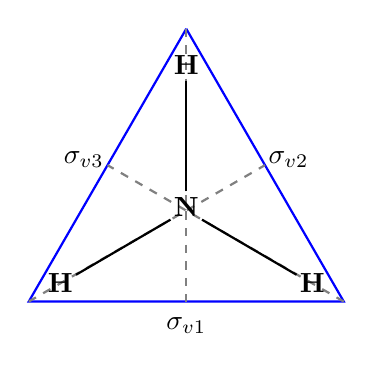
\begin{tikzpicture}[scale=2]
                    \coordinate (one) at (0,1.732);
                    \coordinate (two) at (1,0);
                    \coordinate (three) at (-1,0);
                    \coordinate (onetwo) at (0.5,0.866);
                    \coordinate (twothree) at (0,0);
                    \coordinate (onethree) at (-0.5,0.866);
                    \draw [blue,thick] (one)--(two)--(three)--(one);
                    \draw [gray,thick,dashed] (one)--(twothree);
                    \draw [gray,thick,dashed] (two)--(onethree);
                    \draw [gray,thick,dashed] (three)--(onetwo);
                    \draw [black,thick,solid] (0,0.7)--(0,1.4);
                    \draw [black,thick,solid] (-0.1,0.52)--(-0.7,0.17);
                    \draw [black,thick,solid] (0.1,0.52)--(0.7,0.17);
                    \node at (0,-0.15) {$\sigma_{v1}$};
                    \node at (0.65,0.9) {$\sigma_{v2}$};
                    \node at (-0.65,0.9)
                    {$\sigma_{v3}$};
                    \node at (0,0.6) {\textbf N};
                    \node at (0,1.5) {\textbf H};
                    \node at (-0.8,0.12) {\textbf H};
                    \node at (0.8,0.12) {\textbf H};
                \end{tikzpicture}\\
                \begin{tabular}{l}
                    $E$: Identity\\
                    $C_3$: $120^{\circ}$, counterclockwise\\
                    $C_3^2$: $240^{\circ}$, counterclockwise
                \end{tabular}
            \end{tabular}
            & \hspace{0.25in} &
            \begin{tabular}{cc|cccccc}
                & & \multicolumn{6}{c}{$g$}\\
                & $f \circ g$ & $E$ & $C_3$ & $C_3^2$ & $\sigma_{v1}$ & $\sigma_{v2}$ & $\sigma_{v3}$\\
                \hline
                \multirow{6}{*}{$f$} & $E$ & $E$ & $C_3$ & $C_3^2$ & $\sigma_{v1}$ & $\sigma_{v2}$ & $\sigma_{v3}$\\
                & $C_3$ & $C_3$ & $C_3^2$ & $E$ & $\sigma_{v3}$ & $\sigma_{v1}$ & $\sigma_{v2}$\\
                & $C_3^2$ & $C_3^2$ & $E$ & $C_3$ & $\sigma_{v2}$ & $\sigma_{v3}$ & $\sigma_{v1}$\\
                & $\sigma_{v1}$ & $\sigma_{v1}$ & $\sigma_{v2}$ & $\sigma_{v3}$ & $E$ & $C_3$ & $C_3^2$\\
                & $\sigma_{v2}$ & $\sigma_{v2}$ & $\sigma_{v3}$ & $\sigma_{v1}$ & $C_3^2$ & $E$ & $C_3$\\
                & $\sigma_{v3}$ & $\sigma_{v3}$ & $\sigma_{v1}$ & $\sigma_{v2}$ & $C_3$ & $C_3^2$ & $E$
            \end{tabular}
        \end{tabular}
        \caption{The Cayley table for the $C_{3v}$ point group, using ammonia (\ch{NH3}) as an example. The viewpoint of the molecule is with the nitrogen atom in the plane of the paper and the hydrogen atoms facing away from the reader.}
        \label{tab:c3vcayley}
    \end{table}

    We will do the same process with $C_{2v}$. Clearly, $C_{2v}$ has the identity operation $E$. The $C_2$ rotation is its own inverse, as $C_2C_2=C_2^2=E$. The reflections $\sigma_{v1}$ and $\sigma_{v2}$ are their own inverses. There are $4$ symmetry operations in $C_{2v}$: $\{E, C_2, \sigma_{v1}, \sigma_{v2}\}$. The Cayley table for $C_{2v}$ is shown in Table \ref{tab:c2vcayley}. Closure can be verified from the Cayley table, and associativity follows from the associativity of function composition. Furthermore, from the Cayley table, we can see that the $C_{2v}$ is isomorphic to the Klein 4-group $V_4$.

    \begin{table}[htb]
        \centering
        \renewcommand{\arraystretch}{1.5}
        \begin{tabular}{lcr}
            \begin{tabular}{l}
                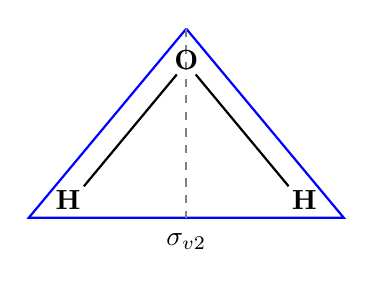
\begin{tikzpicture}[scale=2]
                    \coordinate (one) at (0,1.2);
                    \coordinate (two) at (1,0);
                    \coordinate (three) at (-1,0);
                    \coordinate (onetwo) at (0.5,0.866);
                    \coordinate (twothree) at (0,0);
                    \coordinate (onethree) at (-0.5,0.866);
                    \draw [blue,thick] (one)--(two)--(three)--(one);
                    \draw [gray,thick,dashed] (one)--(twothree);
                    \draw [black,thick,solid] (-0.06,0.91)--(-0.65,0.2);
                    \draw [black,thick,solid] (0.06,0.91)--(0.65,0.2);
                    \node at (0,-0.15) {$\sigma_{v2}$};
                    \node at (0,1) {\textbf O};
                    \node at (-0.75,0.11)
                    {\textbf H};
                    \node at (0.75,0.11)
                    {\textbf H};
                \end{tikzpicture}\\
                \begin{tabular}{l}
                    $E$: Identity\\
                    $C_2$: $180^{\circ}$\\
                    $\sigma_{v1}$: Reflection over molecular plane
                \end{tabular}
            \end{tabular}
            & \hspace{0.25in} &
            \begin{tabular}{cc|cccc}
                & & \multicolumn{4}{c}{$g$}\\
                & $f \circ g$ & $E$ & $C_2$ & $\sigma_{v1}$ & $\sigma_{v2}$\\
                \hline
                \multirow{4}{*}{$f$} & $E$ & $E$ & $C_2$ & $\sigma_{v1}$ & $\sigma_{v2}$\\
                & $C_2$ & $C_2$ & $E$ & $\sigma_{v2}$ & $\sigma_{v1}$\\
                & $\sigma_{v1}$ & $\sigma_{v1}$ & $\sigma_{v2}$ & $E$ & $C_2$\\
                & $\sigma_{v2}$ & $\sigma_{v2}$ & $\sigma_{v1}$ & $C_2$ & $E$
            \end{tabular}
        \end{tabular}
        \caption{The Cayley table for the $C_{2v}$ point group, using water (\ch{H2O}) as an example.}
        \label{tab:c2vcayley}
    \end{table}
    \pagebreak

    \section{Representation of symmetry operations as matrices}

    Our next step in the mathematical analysis is to find matrix representations of the symmetry operations $E$, $C_n$, $\sigma$, $i$, and $S_n$. We will define these operations as transformations of the coordinate vector $(x,y,z)^T$. The identity operation $E$ is represented by the identity matrix \[M_E=\begin{pmatrix}1&0&0\\0&1&0\\0&0&1\end{pmatrix}.\] The rotation operation $C_n$, where the rotation is about the $z$ axis, is represented by the matrix \[M_{C_n}=\begin{pmatrix}\cos\theta&-\sin\theta&0\\\sin\theta&\cos\theta&0\\0&0&1\end{pmatrix},\] where $\theta=\dfrac{360^\circ}{n}$ (bond angles in chemistry are typically expressed in degrees). Matrices for other rotational axes can be constructed similarly. The reflection operations $\sigma$ over the $xy$, $yz$, and $xz$ planes are represented by the respective matrices \[M_{\sigma_{xy}}=\begin{pmatrix}1&0&0\\0&1&0\\0&0&-1\end{pmatrix}, M_{\sigma_{yz}}=\begin{pmatrix}-1&0&0\\0&1&0\\0&0&1\end{pmatrix}, \text{ and }M_{\sigma_{xz}}=\begin{pmatrix}1&0&0\\0&-1&0\\0&0&1\end{pmatrix}.\] The inversion operation $i$ is represented by the matrix \[M_i=\begin{pmatrix}-1&0&0\\0&-1&0\\0&0&-1\end{pmatrix}.\] Finally, the rotation-reflection operation $S_n$, where the rotation is about the $z$ axis and the reflection is over the $xy$ plane, is represented by the matrix \[M_{S_n}=\begin{pmatrix}\cos\theta&-\sin\theta&0\\\sin\theta&\cos\theta&0\\0&0&-1\end{pmatrix},\] where $\theta=\dfrac{360^\circ}{n}$. Matrices for other rotational axes and reflection planes can be constructed similarly.
    
    Now that we have a set of matrices for the symmetry operations, we can express the matrix representation of each of the point groups. To simplify the discussion, we will limit ourselves to the $C_{2v}$ and $C_{3v}$ point groups. We will look at the matrix representation for $C_{2v}$ (\ch{H2O}) first. We use the notation established in Table \ref{tab:c2vcayley}. By convention, we define the $z$ axis as the principal axis and the $xz$ plane as the plane of the molecule, with the oxygen atom at the origin, as shown:

    \begin{center}\includegraphics[width=1.5in]{waterxyz.png}\end{center}
    
    Then the matrices for the symmetry operations of $C_{2v}$ are \[M_E=\begin{pmatrix}1&0&0\\0&1&0\\0&0&1\end{pmatrix}, M_{C_2}=\begin{pmatrix}-1&0&0\\0&-1&0\\0&0&1\end{pmatrix}, M_{\sigma_{v1}}=\begin{pmatrix}1&0&0\\0&-1&0\\0&0&1\end{pmatrix}, \text{ and } M_{\sigma_{v2}}=\begin{pmatrix}-1&0&0\\0&1&0\\0&0&1\end{pmatrix}.\] Multiplying these matrices reveals the same group structure as shown in Table \ref{tab:c2vcayley}.
    
    Now we will look at the matrix representation for $C_{3v}$ (\ch{NH3}). We use the notation established in Table \ref{tab:c3vcayley}. By convention, we define the $z$ axis as the principal axis, the $xy$ plane as parallel to the hydrogen triangle, and the $xz$ plane coinciding with one of the three $\sigma_v$ mirror planes, with the nitrogen atom at the origin, as shown:
    
    \begin{center}\includegraphics[width=1.5in]{ammoniaxyz.png}\end{center}
    
    Then the matrices for the symmetry operations of $C_{3v}$ are \[M_E=\begin{pmatrix}1&0&0\\0&1&0\\0&0&1\end{pmatrix}, M_{C_3}=\begin{pmatrix}-\frac12&-\frac{\sqrt{3}}2&0\\\frac{\sqrt{3}}2&-\frac12&0\\0&0&1\end{pmatrix}, M_{C_3^2}=\begin{pmatrix}-\frac12&\frac{\sqrt{3}}2&0\\-\frac{\sqrt{3}}2&-\frac12&0\\0&0&1\end{pmatrix},\]
    \[M_{\sigma_{v1}}=\begin{pmatrix}1&0&0\\0&-1&0\\0&0&1\end{pmatrix}, M_{\sigma_{v2}}=\begin{pmatrix}-\frac12&-\frac{\sqrt{3}}2&0\\-\frac{\sqrt3}2&\frac12&0\\0&0&1\end{pmatrix}, \text{ and } M_{\sigma_{v3}}=\begin{pmatrix}-\frac12&\frac{\sqrt{3}}2&0\\\frac{\sqrt3}2&\frac12&0\\0&0&1\end{pmatrix}.\] Multiplying these matrices reveals the same group structure as shown in Table \ref{tab:c3vcayley}.

    \section{Characters and reducible/irreducible representations}

    Constructing the matrices for the point groups above was challenging, especially in the case of $C_{3v}$, mainly because appropriate bases needed to be chosen, and the symmetries with respect to those bases needed to be computed with tedious hand calculations. Of course, different bases could have been used, which makes the matrix representations non-unique. These problems are disappointing, especially considering that $C_{2v}$ and $C_{3v}$ are two of the simplest and most common point groups in chemistry!
    
    Thankfully, we have that the trace (character) of a matrix is conjugation invariant. Thus, if we change the basis, the characters remain the same. To simplify the representation of each point group, we will use characters instead of matrices. Quick calculations show that the characters of the symmetry operations in $C_{2v}$ are $\chi_E = 3$, $\chi_{C_2}=-1$, $\chi_{\sigma_{v1}}=1$, and $\chi_{\sigma_{v2}}=1$. The characters in $C_{3v}$ are $\chi_E=3$, $\chi_{C_3}=0$, $\chi_{C_3^2}=0$, $\chi_{\sigma_{v1}}=1$, $\chi_{\sigma_{v2}}1$, and $\chi_{\sigma_{v3}}=1$.

    The conjugacy classes in $C_{2v}$ are the singleton sets $\{E\}, \{C_2\}, \{\sigma_{v1}\}, \{\sigma_{v2}\}$, which follows since $C_{2v}\cong V_4$ is an abelian group. The conjugacy classes in $C_{3v}$ are the sets $\{E\}, \{C_3,C_3^2\},$ and $\{\sigma_{v1},\sigma_{v2},\sigma_{v3}\}$. Every symmetry operation in the same conjugacy class has the same character, and the operations in the same class will be grouped together when we create character tables.

    The characters listed above for $C_{2v}$ and $C_{3v}$ are reducible representations. We will denote reducible representations by $\Gamma$. Our goal is to decompose these reducible representations into irreducible representations (irreps). The irreps will be denoted using a standard notation system.

    One dimensional irreps are denoted $A$ if the representation is symmetric to the principal rotation (that is, $\chi_{C_n}=1$) and $B$ if the representation is antisymmetric to the principal rotation ($\chi_{C_n}=-1$). Two dimensional irreps are denoted $E$, and three dimensional irreps are denoted $T$. Furthermore, subscripts are used to distinguish irreps with the same letter label, and these subscripts are not arbitrary. Subscript 1 is used for an irrep that is symmetric to a perpendicular $C_2$ axis, and subscript 2 is used for an irrep that is antisymmetric to a perpendicular $C_2$. If there is no perpendicular $C_2$ axis, the subscript is determined based on the symmetry (1) or antisymmetry (2) with respect to the vertical mirror plane $xz$. Subscript $g$ (\emph{gerade}) is used for an irrep symmetric to inversion, and $u$ (\emph{ungerade}) is used in the antisymmetric case. For further distinction, $'$ is used for symmetry with respect to $\sigma_h$ and $''$ is used for antisymmetry with respect to $\sigma_h$.
    
    \section{Character tables}

    Character tables are important in chemistry because they provide all of the symmetry information in a given point group in a succinct way. By reading a character table, a chemist can quickly determine which vibrational modes are IR- or Raman- active, the chirality of a molecule, or the way molecular orbitals can form, without needing to perform calculations. In a sense, they ``prepackage'' the underlying group theory into an easily read table that is shared by every molecule in a given point group. We will look at the construction of some simple character tables, and then we will explore some of their applications.

    Now that we have found the matrices for the point groups $C_{2v}$ and $C_{3v}$, we are ready to begin constructing the character table for those point groups, starting with $C_{2v}$. We now revisit the matrices for the $C_{2v}$ symmetry operations, this time block diagonalized: \[M_E=\begin{pmatrix}\boxed1&0&0\\0&\boxed1&0\\0&0&\boxed1\end{pmatrix}, M_{C_2}=\begin{pmatrix}\boxed{-1}&0&0\\0&\boxed{-1}&0\\0&0&\boxed1\end{pmatrix}, M_{\sigma_{v1}}=\begin{pmatrix}\boxed1&0&0\\0&\boxed{-1}&0\\0&0&\boxed1\end{pmatrix}, \text{ and } M_{\sigma_{v2}}=\begin{pmatrix}\boxed{-1}&0&0\\0&\boxed1&0\\0&0&\boxed1\end{pmatrix}.\]

    We start building a character table by placing the elements from the first block in the first row ($x$), the elements from the second block in the second row ($y$), and the elements from the third block in the third row ($z$), and labeling the rows by the aforementioned rules. (Note that the $xz$ plane of the water molecule drawn above corresponds to $\sigma_{v1}$ in Table \ref{tab:c2vcayley}, which distinguishes $B_1$ and $B_2$.) The last two columns will be expanded upon later and their importance will become apparent. Also, there is an empty row which will be filled in soon.

    \begin{table}[htbp]
        \centering
        \renewcommand{\arraystretch}{1.5}
        \begin{tabular}{c|cccc|c|c}
            $C_{2v}$ & $E$ & $C_2$ & $\sigma_{v1}~(xz)$ & $\sigma_{v2}~(yz)$ & ~~~~~~~ & ~~~~~~~\\
            \hline
            $B_1$ & 1 & -1 & 1 & -1 & $x$ &\\
            $B_2$ & 1 & -1 & -1 & 1 & $y$ &\\
            $A_1$ & 1 & 1 & 1 & 1 & $z$ &\\
            &&&&&&\\
            \hline
            $\Gamma$ & 3 & -1 & 1 & 1 & &
        \end{tabular}
    \end{table}

    Character tables have several important properties. Let $\chi_i(C)$ represent the character of class $C$ in the $i$th irrep.
    
    \begin{itemize}
        \item The number of symmetry operations is the order of the group, $h$.
        \item If symmetry operations are grouped by conjugacy class $C$, we show how many operations are in the class, $n_C$, in the top row. For example, if there are three rotations in the $C_2$ class, the top row will be labeled $3C_2$. We will call $n_C$ the multiplicity of the class.
        \item The number of irreps equals the number of classes. That is, the character table needs to have the same number of rows and columns.
        \item Taking the sum over all of the irreps, we have \[\sum_i\chi_i^2(E)=h,\] where $E$ is the identity operation.
        \item For the $i$th irrep, we have \begin{equation}\sum_C n_C \chi_i^2(C)=h,\label{sumsq}\end{equation} where the sum is taken over all of the conjugacy classes.
        \item \textbf{Orthogonality Theorem.} Irreps are orthogonal. We have, for the $i$th and $j$th irreps, \begin{equation}
        \sum_C n_C \chi_i(C)\chi_j(C)=h\delta_{ij},\label{orthog}\end{equation} where $\delta_{ij}$ is the Kronecker delta. This form of the orthogonality formula is easily proven from the fact that every symmetry operation in a given conjugacy class has the same character. When $i=j$, \eqref{orthog} reduces to \eqref{sumsq}, and when $i\neq j$, we have \[\sum_C n_C \chi_i(C)\chi_j(C)=0.\] 
        \item One irrep has characters that are all $1$, which is labeled $A_1$.
        \item Each irrep must be distinct.
    \end{itemize}

    Applying these rules, we deduce that there is indeed a fourth irrep, and using the Orthogonality Theorem along with the other properties, we can find the characters of this fourth irrep, $A_2$.

    \begin{table}[htbp]
        \centering
        \renewcommand{\arraystretch}{1.5}
        \begin{tabular}{c|cccc|c|c}
            $C_{2v}$ & $E$ & $C_2$ & $\sigma_{v1}~(xz)$ & $\sigma_{v2}~(yz)$ & &\\
            \hline
            $A_1$ & 1 & 1 & 1 & 1 & $z$ & $x^2, y^2, z^2$\\
            $A_2$ & 1 & 1 & -1 & -1 & $R_z$ & $xy$\\
            $B_1$ & 1 & -1 & 1 & -1 & $x, R_y$ & $xz$\\
            $B_2$ & 1 & -1 & -1 & 1 & $y, R_x$ & $yz$\\
        \end{tabular}
    \end{table}

    We now have a complete character table for $C_{2v}$. Notice that additional information has been added to the last two columns. The symbols $R_x$, $R_y$, and $R_z$ indicate the irreps that match the symmetry or antisymmetry of rotations about the $x$, $y$, and $z$ axes, respectively. For example, the $C_2$ operation corresponds to the $R_z$ rotation, and the $A_2$ irrep is symmetric with respect to $C_2$. Thus, the $A_2$ row gets $R_z$. The $\sigma_{v1}$ operation corresponds to a reflection over the $xz$ plane, which is perpendicular to the $y$ axis, and the $B_1$ irrep is symmetric with respect to $\sigma_{v1}$. Thus, the $B_1$ row gets $R_y$. The $B_2$ row gets $R_x$ similarly. The symbols $x^2$, $y^2$, $xy$, etc. represent mathematical functions that are symmetric with respect to the irreps. For instance, we know that the product function $xy$ is positive in the first and third quadrants and negative in the second and fourth quadrants, and a $180^\circ$ rotation about the $z$ axis maintains these signs. However, a $180^\circ$ rotation about the $x$ or $y$ axes reverses these signs. Hence, $xy$ appears in the same row as $R_z$. Note that $xy$ and $R_z$ remain unchanged under $C_2$ and change sign with reflection over either mirror plane. The functions $x^2$, $y^2$, and $z^2$ are always positive, so they are symmetric with respect to the $A_1$ irrep.

    At first, it may seem like these last two columns are only for curiosity's sake. However, as we will see, they have important applications in chemistry.

    Now we will construct a character table for the $C_{3v}$ point group. We now revisit the matrices for the $C_{3v}$ symmetry operations, this time block diagonalized: \[M_E=\left(\begin{array}{cc|c}1&0&0\\0&1&0\\\hline0&0&1\end{array}\right), M_{C_3}=\left(\begin{array}{cc|c}-\frac12&-\frac{\sqrt{3}}2&0\\\frac{\sqrt{3}}2&-\frac12&0\\\hline0&0&1\end{array}\right), M_{C_3^2}=\left(\begin{array}{cc|c}-\frac12&\frac{\sqrt{3}}2&0\\-\frac{\sqrt{3}}2&-\frac12&0\\\hline0&0&1\end{array}\right),\]
    \[M_{\sigma_{v1}}=\left(\begin{array}{cc|c}1&0&0\\0&-1&0\\\hline0&0&1\end{array}\right), M_{\sigma_{v2}}=\left(\begin{array}{cc|c}-\frac12&-\frac{\sqrt{3}}2&0\\-\frac{\sqrt3}2&\frac12&0\\\hline0&0&1\end{array}\right), \text{ and } M_{\sigma_{v3}}=\left(\begin{array}{cc|c}-\frac12&\frac{\sqrt{3}}2&0\\\frac{\sqrt3}2&\frac12&0\\\hline0&0&1\end{array}\right).\]

    The $C_3$ and $C_3^2$ operations are in the same class, and likewise the three $\sigma_v$ operations are in the same class, so they will be grouped together in the character table.

    Following the procedure established above, we will go ahead and create the full character table for $C_{3v}$.
    
    \begin{table}[htbp]
        \centering
        \renewcommand{\arraystretch}{1.5}
        \begin{tabular}{c|ccc|c|c}
            $C_{3v}$ & $E$ & $2C_3$ & $3\sigma_{v}$ & &\\
            \hline
            $A_1$ & 1 & 1 & 1 & $z$ & $x^2+y^2, z^2$\\
            $A_2$ & 1 & 1 & -1 & $R_z$ &\\
            $E$ & 2 & -1 & 0 & $(x,y), (R_x,R_y)$ & $(x^2-y^2,xy),(xz,yz)$\\
        \end{tabular}
    \end{table}

    We can verify that the order relations and orthogonality relations hold. For instance, $2^2+2(-1)^2+3(0)^2=6$, and $1\cdot2 + 2(1\cdot-1) + 3(-1\cdot0) = 0$. Furthermore, notice that the label $E$ was used for the two-dimensional irrep (2 in the $E$ identity operation column). Confusingly, in chemistry, $E$ is used to represent both the identity operation and 2D irreps. Also, notice that in the list of functions on the right, we group $x$ and $y$ together in parentheses. This is based on the block diagonalization, where $x$ and $y$ together form one block and $z$ individually forms another block.

    \section{Expressing reducible representations in terms of irreps}

    The reducible representation $\Gamma$ can be written as a linear combination of the irreducible representations (irreps). That is, for each class $C$, and for each character $\chi(C)$ in $\Gamma$, with corresponding character $\chi_i(C)$ in the $i$th irrep, there exist coefficients $n_1, n_2,\ldots$ such that \begin{equation}\chi_C=\sum_in_i\chi_i(C).\label{lincomb}\end{equation}
    
    \textbf{Lemma 1.} Each coefficient $n_i$ in \eqref{lincomb} is given by
    \[n_i=\frac1h\sum_Cn_C\chi(C)\chi_i(C),\]
    where $h$ is the order of the group.

    \begin{proof}
        From the Orthogonality Theorem, we have, for the $i$th and $j$th irreps, \[\sum_C n_C \chi_i(C)\chi_j(C)=h\delta_{ij}.\]
        Taking the sum over all $j$ irreps, and multiplying both sides by $n_j$, we have \begin{equation}\sum_C n_C\sum_jn_j \chi_i(C)\chi_j(C)=h\sum_jn_j\delta_{ij}=hn_i.\label{lemmastep2}\end{equation}
        We have by \eqref{lincomb} that $\sum_jn_j\chi_j(C)=\chi(C)$. Substituting into \eqref{lemmastep2}, we get \[\sum_C n_C\chi(C)\chi_i(C)=hn_i.\] Divide both sides by $h$ to complete the proof.
    \end{proof}
    
    We can use Lemma 1 to find the number of times that an irrep contributes to $\Gamma$. We will look at an application of Lemma 1 in the next section, where we consider the vibrations of the water molecule.


    \section{Molecular vibrations}

    Not only do molecules as a whole move around, but also the individual atoms can move around slightly within the molecule, producing molecular vibrations. To mathematically study these vibrations, we need to first assign a separate 3D coordinate axis to each atom. For a molecule with $N$ atoms, each atom can move independently in three dimensions, so there are $3N$ possible motions, called \emph{degrees of freedom}.

    In a nonlinear molecule, there are three translational \emph{modes}, three rotational modes, and the remaining $3N-6$ modes are vibrational. In a linear molecule, there are also three translational modes. However, a linear molecule only has two rotational modes, since a rotation along the axis of the molecule does not change the relative orientation of the atoms. Then the remaining $3N-5$ modes are vibrational.

    If we create a $3N\times3N$ transformation matrix to represent the effect of a symmetry operation on the position of each atom, an element in the diagonal of the matrix will be 1 if the atom remains in its original location, -1 if it reverses direction, and 0 if it moves. We can then take the character of the matrix for each symmetry operation. Since operations in the same class have the same character, we only need to construct one such matrix for each class. However, constructing these matrices explicitly can be tedious, especially for a molecule with many atoms. Thankfully, the only information we need from these matrices is their characters, and we can find the characters without explicitly constructing the matrices.

    We will use the vibrations of the water molecule as an example. For convenience, we stick with the same coordinate axes that were used above, such that the $z$ axis is the principal axis and the $xz$ plane is the plane of the molecule. This time, however, each atom gets its own set of coordinate axes, and each atom is considered to be at its own origin. Since water has three atoms (one oxygen and two hydrogens), it has nine degrees of freedom.

    Since water is a nonlinear molecule, it has $3N-6=3$ vibrational modes. One of these is \emph{symmetric stretch}, where the lengths of the \ch{O-H} bonds lengthen and shorten in unison. One is \emph{antisymmetric stretch}, where one \ch{O-H} bond lengthens as the other one shortens. The last one is \emph{symmetric bend}, where the bond angle increases and decreases, similar to a bird flapping its wings. Each of these vibrational modes changes the \emph{dipole moment} of water, causing its polarity to oscillate slightly. If a picture is worth a thousand words, an animation is worth a million. The vibrational modes of water (and other molecules) can be seen at \url{https://www.chem.purdue.edu/jmol/vibs/h2o.html}.

    We could create a $9\times 9$ transformation matrix for each of the four symmetry classes in water. However, we can find the characters of each matrix without explicitly constructing the matrices. In the identity operation $E$, every atom remains in the same position, so the character $\chi_E=9$. In the rotation $C_2$, the hydrogen atoms both move, so they contribute nothing to the character. The oxygen atom reverses direction with respect to $x$ $(-1)$ and $y$ $(-1)$, but not with respect to $z$ $(1)$. Thus, oxygen contributes a net of $-1$ to the character. Hence $\chi_{C_2}=-1$. In the reflection $\sigma_{v1}~(xz)$, in the plane of the molecule, the $x$ and $z$ directions stay the same for each atom, while the $y$ direction flips for each atom. Then $\chi_{\sigma_{v1}}=3-3+3=3$. In the reflection $\sigma_{v2}~(yz)$, the hydrogen atoms swap positions, so they contribute nothing to the character. The oxygen atom reverses direction with respect to $x$ $(-1)$ but not with respect to $y$ $(1)$ or $z$ $(1)$. Therefore, $\chi_{\sigma_{v2}}=1$. We are now ready to show the full $C_{2v}$ character table again, this time with $\Gamma$ included.

    \clearpage

    \begin{table}[htbp]
        \centering
        \renewcommand{\arraystretch}{1.5}
        \begin{tabular}{c|cccc|c|c}
            $C_{2v}$ & $E$ & $C_2$ & $\sigma_{v1}$ & $\sigma_{v2}$ & &\\
            \hline
            $A_1$ & 1 & 1 & 1 & 1 & $z$ & $x^2, y^2, z^2$\\
            $A_2$ & 1 & 1 & -1 & -1 & $R_z$ & $xy$\\
            $B_1$ & 1 & -1 & 1 & -1 & $x, R_y$ & $xz$\\
            $B_2$ & 1 & -1 & -1 & 1 & $y, R_x$ & $yz$\\
            \hline
            $\Gamma$ & 9 & -1 & 3 & 1 & &\\
        \end{tabular}
    \end{table}

    We can now use Lemma 1 to express $\Gamma$ as a linear combination of the irreps $A_1, A_2, B_1$, and $B_2$. We have \[n_{A_1}=\frac14((9)(1)+(-1)(1)+(3)(1)+(1)(1))=3.\] Similarly, we calculate $n_{A_2}=1$, $n_{B_1}=3$, and $n_{B_2}=2$. We find that \begin{equation}\Gamma = 3A_1+A_2+3B_1+2B_2.\label{linearcombo}\end{equation} Looking at the character table, the three translational modes of a $C_{2v}$ molecule like water correspond to the irreps that have $x$, $y$, or $z$ listed on the right hand side, so the three translational modes correspond to the irreps $A_1$, $B_1$, and $B_2$. The three rotational modes correspond to the irreps that have $R_x$, $R_y$ and $R_z$ listed, which are $A_2$, $B_1$, and $B_2$. Taking \eqref{linearcombo} and subtracting $A_1 + B_1 + B_2 + A_2 + B_1 + B_2$, for the translational and rotational modes, we have $2A_1+B_1$ remaining, which are the three vibrational modes. Two correspond to the $A_1$ irrep and one corresponds to the $B_1$ irrep. This will be important in the next section.

    For other molecules besides water, we do a similar process. We consider the effect of each symmetry operation on each atom in order to determine the characters of each class. Using Lemma 1, we express $\Gamma$ as a linear combination of the irreps. From this linear combination, we subtract the irreps that correspond to translational or rotational modes (the ones that have $x, y, z, R_x, R_y, \text{ or } R_z$ listed) to find the number of vibrational modes that correspond to each irrep.

    \section{Applications: Spectroscopy}

    Much information can be determined about a molecule based on how it absorbs infrared light at various wavelengths. IR spectroscopy is a very common technique to ``draw a picture'' of a molecule in order to learn about the bonds and groups of atoms present. In Figure \ref{fig:irwater}, we see a labeled IR spectrum of water.

    \begin{figure}[htbp]
        \centering
        \includegraphics[width=6in]{irwater.png}
        \caption{IR spectrum of water, showing the characteristic peaks of its IR active vibrational modes. \cite{gutow2015}}
        \label{fig:irwater}
    \end{figure}

    When a molecule absorbs light in the infrared region of the spectrum, vibrations that result in a change of dipole moment are affected. As we said earlier, the three vibrational modes of water (symmetric stretch, antisymmetric stretch, and symmetric bend) all impact the dipole moment of water, so they appear in the IR spectrum. (The two stretch bands are so close together and broad that they merge into one large peak.) Interestingly, even though carbon dioxide (\ch{CO2}) is nonpolar by linear symmetry, when it absorbs infrared light, it will vibrate in such a way as to momentarily break the linear symmetry and make \ch{CO2} slightly polar! This is why \ch{CO2} absorbs infrared light, making it a greenhouse gas. \cite{royal2009}

    How do we know which vibrational modes affect the dipole moment and are thus represented by peaks in the IR spectrum? That is to say, which vibrations are \emph{IR active}? Well, we just need to look at the character table and see which irreps have the same symmetry as $x$, $y$, or $z$. In the last section, we determined that water has two vibrational modes corresponding to the irrep $A_1$ and one corresponding to the irrep $B_1$. We see that $A_1$ has the same symmetry as $z$ and $B_1$ has the same symmetry as $x$, so all three vibrational modes of water are IR active. This makes sense, since we said earlier that each of the vibrational modes of water changes the dipole moment! If there were a vibrational mode corresponding to, say, the $A_2$ irrep, then that mode would be \emph{IR inactive} and not appear on an IR spectrum. But we have mathematically eliminated that possibility for water.

    Raman spectroscopy is similar to IR spectroscopy, but using a different approach. High energy light bombards the molecules, putting them into an excited state temporarily. When they relax back to their various vibrational energy states, they release radiation that can be detected. A vibrational mode is \emph{Raman active} if it exhibits a change of polarizability, which is the tendency to acquire a dipole moment from an electric field. To determine which vibrational modes are Raman active, we look for those irreps that have the same symmetry as $x^2$, $y^2$, $z^2$, $xy$, $yz$, or $xz$, or a linear combination of those. All of the vibrational modes of water are Raman active, which we can determine quickly from the $C_{2v}$ character table.

    \section{Applications: Chirality}

    Our hands are mirror images of each other, but they are not superimposable. Likewise, \emph{chiral} molecules are those that are non-superimposable over their mirror images, as in Figure \ref{fig:enantiomers}. When an atom is bonded to four distinct atoms or clusters of atoms, the molecule is chiral. Each configuration is called an \emph{enantiomer}. A molecule that is not chiral is \emph{achiral}.

    \begin{figure}[ht]
        \centering
        \includegraphics[width=3in]{enantiomers.png}
        \caption{Chiral molecules are non-superimposable over their mirror images. Notice that it is impossible to rotate the molecule on the left to look exactly like the molecule on the right. \cite{monash}}
        \label{fig:enantiomers}
    \end{figure}

    Chiral compounds may occur in \emph{racemic mixtures} where 50\% is in the one enantiomer and 50\% is in the other. However, if plane-polarized light is passed through a sample of a chiral substance consisting of an unequal balance of the enantiomers, the direction of the light will rotate, as in Figure \ref{fig:chiral}. This is called \emph{optical activity}. The two enantiomers rotate light in opposite directions. This is the principle behind how liquid crystal displays (LCDs) work! \cite{lininger2022}

    \begin{figure}[htbp]
        \centering
        \includegraphics[width=3.5in]{chiral.jpg}
        \caption{Chiral compounds that consist of an unequal mixture of enantiomers rotate plane-polarized light. \cite{halpern}}
        \label{fig:chiral}
    \end{figure}

    Interestingly, the pain reliever ibuprofen is a chiral molecule. It is sold as a racemic mixture, although only one of its enantiomers is effective. Furthermore, the drug thalidomide is chiral. One of its enantiomers is a sedative, while the other causes extreme birth defects. \cite{jonsson2017}

    If a molecule contains any $\sigma_h, \sigma_v, \sigma_d, S_n$, or $i$ symmetry elements, it is achiral. Hence, the only symmetries possible for a chiral compound are the identity $E$ and proper rotation axes $C_n$. A chiral molecule cannot have a mirror plane, improper rotation axis, or center of inversion. If a molecule has a mirror plane \emph{and} a center of inversion, it must also have an improper rotation axis. Therefore, any molecule that belongs to a point group that does not have $S_n$ is chiral. A look at the character table of a molecule's point group will tell which symmetry elements are present, from which one can deduce that the molecule is chiral or achiral.

    \section{Conclusion}

    We have only begun to scratch the surface of the intricate links between symmetry and chemistry. A full development of molecular theory would not be possible without an algebraic treatment of symmetry. As we have seen, character tables provide a unique and readable ``fingerprint'' of point groups, eliminating the need to describe each molecule individually from a group-theoretic standpoint. From the table, much information can be quickly inferred, such as the numbers and types of symmetries present, IR/Raman activity, and chirality. This beautiful area of study ties together chemistry, geometry, group theory, representation theory, and linear algebra. I hope you have enjoyed reading this paper as much as I have enjoyed creating it!

    \printbibliography[heading=bibnumbered]
\end{document}